\documentclass[a4paper,10pt]{article}
\usepackage{amsmath}
\usepackage{mathtools}
\usepackage{cancel}
\usepackage{amsfonts}
\usepackage{amssymb}
\usepackage{graphicx}
\usepackage{siunitx}
\usepackage{physics}
\usepackage{nicefrac}
\usepackage{unicode-math}
\usepackage{tikz}
\usepackage{circuitikz}
\ctikzset{bipoles/length=0.75cm}
\ctikzset{american voltages}
\ctikzset{american currents}

\usepackage{fontspec}
\usepackage[activate={true,nocompatibility},final,tracking=true,factor=1100,stretch=20,shrink=20]{microtype}

\setmainfont[Renderer=Basic
%, Numbers=OldStyle
,Scale = 1.0
,Ligatures=TeX
]{Linux Libertine}

\newfontfamily\biolinum{Linux Biolinum}

\usepackage{mathrsfs}
\newcommand{\Ham}{\mathscr{H}}

\renewcommand{\descriptionlabel}[1]{\hspace{\labelsep}\textit{\biolinum{#1}}}
\usepackage{titlesec}
\titleformat*{\paragraph}{\large\itshape\biolinum}

\usepackage{geometry}
 \geometry{
 a4paper,
 total={170mm,257mm},
 left=25mm,
 right=25mm,
 top=20mm,
 }


\usepackage[most]{tcolorbox}

\tcbset{
    frame code={}
    center title,
    left=0pt,
    right=0pt,
    top=0pt,
    bottom=0pt,
    colback=blue!10!white,
    colframe=white,
    width=0.5\textwidth,
    enlarge left by=0mm,
    boxsep=5pt,
    arc=0pt,outer arc=0pt,
    }


    % Light the notation
    \newcommand{\kb}{\mathrm{k}}
    \newcommand{\kbt}{\kb T}
    \newcommand{\vbe}{
      \textcolor{green!30!black}
      {
        \left( \mathrm{e}^{qV_{\mathit{BE}}/\kbt} - 1 \right)
      }
    }
    \newcommand{\vbc}{
      \textcolor{red!30!black}
      {
        \left( \mathrm{e}^{qV_{\mathit{BC}}/\kbt} - 1 \right)
      }
    }

\usepackage{multicol}

\newcommand{\coolsection}[1]{
  \begin{tcolorbox}
      \large\biolinum{\textsc{#1}}
  \end{tcolorbox}
}


\begin{document}

\begin{center}
\textsc{\Huge Semiconductors 101}

\textit{``Oops! I did it again''}
\end{center}

\vspace{0.5cm}

\begin{multicols}{2}
  \coolsection{Hartree-Fock approximation}
  The Hamiltonian contains all the possible interactions between
  electrons an nuclei. We can approximate that to a central potential
  $V(\mathbf{r}_i)$ for each electron:
  \begin{equation*}
    \Ham \simeq \sum_\mathit{i} \frac{-ℏ^2}{2m_i} \nabla_i^2 + V(\mathbf{r}_i)
  \end{equation*}
  This is factorizable, so for each electron
  \begin{equation*}
    \left[ \frac{-ℏ^2}{2m_i} \nabla_i^2 + V(\mathbf{r}_i) \right]
    \Psi_i = E_i \Psi_i
  \end{equation*}
  We use periodic boundary conditions (\textsc{Born-Karman
    conditions}). Tight-binding assumption lets us consider that
  levels are those of the base atom but with extra shifted levels.
  \coolsection{Schrödinger, effective mass}
  If $E\sim E_{\mathit{c}} + \frac{ℏ^2 k^2}{2m^*_\mathit{n}}$ we can neglect $V(r)$ and
  write
  \begin{equation*}
    \frac{-ℏ^2}{2m^*_\mathit{n}}∇Ψ = E'Ψ'
  \end{equation*}
  If $E_{\mathit{D}} \sim E_{\mathit{c}} + E''$, with small $\abs{E''}$, we can neglect the
  $V(r)$ in $\mathcal{V}(r) = V(r) - \frac{q^2}{4πεr}$, and write
  \begin{equation*}
    \left( \frac{-ℏ^2}{2m^*_\mathit{n}}∇- \frac{q^2}{4πεr} \right)Ψ''=E''Ψ''
  \end{equation*}
  For the valence band ($E_{\mathit{A}} \sim E_{\mathit{V}} + E''$),
  \begin{equation*}
    \left( \frac{-ℏ^2}{2m^*_\mathit{p}}∇- \frac{q^2}{4πεr} \right)Ψ''= -E''Ψ''
  \end{equation*}
  using $m^*_\mathit{p}=-m^*_\mathit{n}$ and the fact that the
  potential changes sign.

  The effective mass, $m*_\mathit{n} = \frac{ℏ}{\pdv[2]{E}{k}}$, is positive in
  the border of $E_C, E_V$ next to the Fermi level and negative in the
  opposite one.

  \coolsection{Fermi level}
  Let $N_{\mathit{i}}$ be the effective density of states and $n_0,p_0$ the total
  volume concentrations of charge carriers.
  \paragraph{No doping}
  We obtain
  \begin{align*}
    n_0 &= N_{\mathit{C}} \mathrm{e}^{-ΔE/\kbt} = N_{\mathit{C}} \mathrm{e}^{-(E_{\mathit{C}}-E_{\mathit{F}})/\kbt} \\
    p_0 &= N_{\mathit{V}} \mathrm{e}^{-ΔE/\kbt} = N_{\mathit{V}}
          \mathrm{e}^{-(E_{\mathit{F}}-E_{\mathit{V}})/\kbt} \\
    n_i&= \sqrt{n_0p_0} \propto T^{3/2} \mathrm{e}^{-E_\mathit{G}/2\kbt}
  \end{align*}
  since $n_0=p_0$,
  \begin{equation*}
    E_{\mathit{F}} = \frac{E_{\mathit{V}} + E_{\mathit{C}}}{2} + \cancelto{0}{ \frac{\kb T}{2}\log \left( \frac{N_\mathit{V}}{N_\mathit{C}} \right)^{3/2}}
  \end{equation*}
  The term cancels at $T∼\SI{300}{\kelvin}$.

  \paragraph{N doping}
  $E_{\mathit{F}}$ near $E_{\mathit{C}}$:
  \begin{equation*}
    n_0 = N_{\mathit{D}} = N_{\mathit{C}} \mathrm{e}^{-(E_{\mathit{C}}-E_{\mathit{F}})/\kbt}
  \end{equation*}
  \begin{equation*}
    E_{\mathit{F}} = E_{\mathit{C}} - \kbt \log \frac{N_{\mathit{C}}}{N_{\mathit{D}}}
  \end{equation*}
  \paragraph{P doping}
  $E_{\mathit{F}}$ near $E_{\mathit{V}}$:
  \begin{equation*}
    p_0 = N_{\mathit{A}} = N_{\mathit{V}} \mathrm{e}^{-(E_{\mathit{F}}-E_{\mathit{V}})/\kbt}
  \end{equation*}
  \begin{equation*}
    E_{\mathit{F}} = E_{\mathit{V}} + \kbt \log \frac{N_{\mathit{V}}}{N_{\mathit{A}}}
  \end{equation*}

  \coolsection{Extrinsic semiconductors}
  Suppose $ρ=0=q(N_{\mathit{D}}^+ - N_{\mathit{A}}^- + p_0 - n_0)$.
  \begin{center}
    \begin{tabular}{l|l}
      N type ($N_{\mathit{A}}^- = 0$) & P type ($N_{\mathit{D}}^+ = 0$) \\ \hline

      \parbox{3cm}
      {
      \begin{equation*}
        \begin{split}
          n_0 &= p_0 + N_{\mathit{D}}^+ \\
          &= \frac{n_{\mathit{i}}^2}{n_0} + N_{\mathit{D}}^+
        \end{split}
      \end{equation*}
            }

              &

                \parbox{3cm}
                {
      \begin{equation*}
        \begin{split}
          p_0 &= n_0 + N_{\mathit{A}}^- \\
          &= \frac{n_{\mathit{i}}^2}{p_0} + N_{\mathit{A}}^-
        \end{split}
      \end{equation*}
            }

    \end{tabular}
  \end{center}

  Solve 2\textsuperscript{nd} degree equation, obtaining in the N case:
  \begin{equation*}
    n_0 = \frac{N_{\mathit{D}}^+ \pm \sqrt{(N_{\mathit{D}}^+)^2 + 4n_{\mathit{i}}^2}}{2}
  \end{equation*}
  for $p_0$, the relation $n_0 = p_0 + N_{\mathit{D}}^+$ is used.

  \coolsection{Temperature ranges}
  Considering a N semiconductor, we analyze three regions:
  \begin{description}
  \item[Low temperatures] The number of non-ionized impurities ($N_{\mathit{D}}$)
    is greater than the number $N_{\mathit{D}}^+$ of ionized ones ,
    $N_{\mathit{D}}>N_{\mathit{D}}^+≫2n_{\mathit{i}}$. From this inequality follows $n_0≃N_{\mathit{D}}^+$ and
    $p_0 ≃ n_{\mathit{i}}^2 / N_{\mathit{D}}^+$.
  \item[Extrinsic range] The same reasoning as in the low temperature
    region, but this time \emph{all} the impurities are ionized, so
    $N_{\mathit{D}}≃N_{\mathit{D}}^+$. About \SIrange{150}{400}{\kelvin}.
  \item[High temperatures] $n_{\mathit{i}} ≫ N_{\mathit{D}} = N_{\mathit{D}}^+$, and the expression for
    $n_0$ simplifies to $n_0 ≃ p_0 ≃ n_{\mathit{i}}$.
  \end{description}


  \coolsection{Approximations}
  \begin{description}
  \item[Low level injection] Carrier variations being very small
    compared to $n_0,p_0$ implies that $R-G ∝ n',p'$.
  \item[Quasi-neutrality condition] In low level injection conditions,
    the homogeneous parts of a extrinsic semiconductor can be
    considered neutral, much like a metal.
  \item[Negligible minority carrier drag] When determining the total
    current density, the minority carrier contribution to the drag
    current is negligible. They move mainly through diffusion (drift).
  \end{description}


\end{multicols}






\newpage







\begin{center}
\textsc{\Huge Diodes}

\textit{``When everything else fails''}
\end{center}

\vspace{0.5cm}

\begin{multicols}{2}

  \coolsection{Forces}

  \begin{center}
    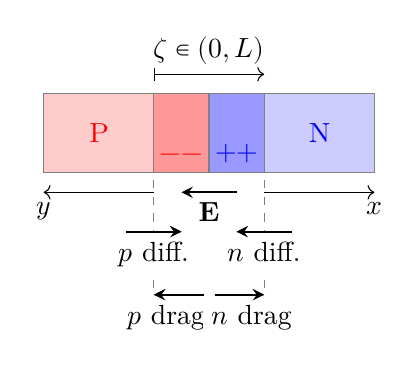
\begin{tikzpicture}[xscale=0.7, yscale=1]
      % Axis and such
      \draw[->] (1,0) -- (3,0)
      node[at end, below] {$x$};
      \draw[->] (-1,0) -- (-3,0)
      node[at end, below] {$y$};
      \draw[|->] (-1,1.5) -- (1,1.5)
      node[above,midway] {$ζ∊(0,L)$};
      \draw[gray,dashed] (1,1) -- (1,-1.5);
      \draw[gray,dashed] (-1,1) -- (-1,-1.5);
      \draw[->,thick,>=stealth] (0.5,-0) -- (-0.5,-0)
      node[below,midway] {$\mathbf{E}$};
      % Chapuza below
      \draw[->,thick,>=stealth] (-1.5,-0.5) -- (-0.5,-0.5)
      node[below,midway,fill=white,minimum size=0.1cm] {$p$ diff.};
      \draw[->,thick,>=stealth] (-1.5,-0.5) -- (-0.5,-0.5);

      \draw[->,thick,>=stealth] (1.5,-0.5) -- (0.5,-0.5)
      node[below,midway,fill=white,minimum size=0.1cm] {$n$ diff.};
      \draw[->,thick,>=stealth] (1.5,-0.5) -- (0.5,-0.5);

      \draw[->,thick,>=stealth] (-0.1,-1.3) -- (-1.0,-1.3)
      node[below,near end,fill=white,minimum size=0.1cm] {$p$ drag};
      \draw[->,thick,>=stealth] (-0.1,-1.3) -- (-1.0,-1.3);

      \draw[->,thick,>=stealth] (0.1,-1.3) -- (1.0,-1.3)
      node[below,near end,fill=white,minimum size=0.1cm] {$n$ drag};
      \draw[->,thick,>=stealth] (0.1,-1.3) -- (1.0,-1.3);
      % Zones
      \draw[thin, gray,fill=red!20!white] (-3,0.25) rectangle
      (-1,1.25); % P
      \draw[thin, gray,fill=red!40!white] (-1,0.25) rectangle
      (0,1.25); % transition P
      \draw[thin, gray,fill=blue!40!white] (0,0.25) rectangle
      (1,1.25); % transition N
      \draw[thin, gray,fill=blue!20!white] (1,0.25) rectangle
      (3,1.25); % N
      % Labels
      \node[below,red] at (-2,1) {\textsc{P}};
      \node[below,blue] at (+2,1) {\textsc{N}};
      \node[above,red] at (-0.5,0.27) {$- -$};
      \node[above,blue] at (+0.5,0.25) {$+ +$};
    \end{tikzpicture}
  \end{center}

  \paragraph{Zero bias} In equilibrium, both forces (drag and drift)
counterbalance. There is no current flow except for the thermal
generation of carriers.

  \paragraph{Forward bias} When a positive voltage bias between
  the P and the N side is applied, holes and electrons recombine and $L$
  gets smaller. $E$ decreases and even changes sign. If the applied $V$
  is big enough, $E$ can not counteract the diffusion of carriers and
  there is a current flow.

  Also, a smaller $L$ increases $∇n,∇p$ in the transition zone and the
  diffusion current, further increasing the conductivity.

  The majority of the current is through drag, so each region
  contributes with its majority carriers, of which it has a constant
  supply from the battery.

  \paragraph{Backward bias} If the bias is negative, $L$ increases
  and there is even less current flow. The only carriers that flow are
  the minoritary ones through diffusion, the ones that the regions
  aren't receiving from the battery. The only source of them is the
  thermal generation, so the current is fixed to a value $I_S \neq f(V)$.

  \coolsection{Analysis}

  Charged currents:
  \begin{align*}
    {\mathbf{J}}_\text{drag} &= qn μ_{\mathit{n}} \mathbf{E},\ qp μ_{\mathit{p}} \mathbf{E}\\
    {\mathbf{J}}_\text{drift} &= qD_{\mathit{n}} ∇n,\ -q D_{\mathit{p}} ∇p\\
    ∇\mathbf{J} &= q (G-R)
  \end{align*}

  Continuity equation:
  \begin{align*}
    \dot{n}_{\mathit{p}} &= \frac{1}{q} \pdv{J_{\mathit{n}}}{x} + G_{\mathit{n}} - \frac{n_{\mathit{p}}'}{τ_{\mathit{n}}}\\
    \dot{p}_{\mathit{n}} &= \frac{-1}{q} \pdv{J_{\mathit{p}}}{x} + G_{\mathit{p}} - \frac{p_{\mathit{n}}'}{τ_{\mathit{p}}}
  \end{align*}

  \coolsection{Contact potential}
  The transition zone is characterized by a constant charge given
  by ionized impurities.
  ${\eval{\mathbf{J}_{\mathit{n}}}_\text{diff} \simeq -
  \eval{\mathbf{J}_{\mathit{n}}}_\text{drag}}$ implies
  \begin{align*}
    -q n μ_{\mathit{n}} ∇V &\simeq -q D_{\mathit{n}} ∇n \\
    \frac{q}{\kbt} \dd{V} &\simeq \frac{\dd{n}}{n}\\
    n(ζ) &\simeq n(0) \mathrm{e}^{qΦ(ζ) / \kbt}
  \end{align*}
  We have $n(ζ=L)=N_{\mathit{D}} = \frac{n_{\mathit{i}}^2}{N_{\mathit{A}}}$ and
  $n(0)=n_{\mathit{p0}}=\frac{n_{\mathit{i}}^2}{N_{\mathit{A}}}$, so
  \begin{equation*}
    Φ_{\mathit{B}} = \frac{\kbt}{q} \log \frac{N_{\mathit{A}} N_{\mathit{D}}}{n_{\mathit{i}}^2}
  \end{equation*}

  \coolsection{Circuit models}

  \paragraph{Analytical} $I = I_{\mathit{S}} (\mathrm{e}^{qV/n\kbt}-1)$
  \paragraph{DC} If $V>V_{\mathit{u}}$ is
  \raisebox{-2mm}{
    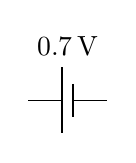
\begin{tikzpicture}[xscale=1,yscale=0.8]
      \draw (0,0)
      to [battery1,l=\SI{0.7}{\V}] (1,0);
    \end{tikzpicture}
    }, else is a open circuit. If a Zener diode is employed, below
    $V_{\mathit{z}}$ it can be modeled by a battery of
    $V=V_{\mathit{z}}$. In both batteries the diode current flows from
    $+$ to $-$.
    \paragraph{AC} The notation is
    \begin{equation*}
      \underbrace{v_{\mathit{D}}}_{\text{Total}} = \underbrace{V_{\mathit{D}}}_{\text{DC}}
      + \underbrace{v_{\mathit{d}}}_{\text{AC}}
    \end{equation*}
    The diode (if not in open circuit) is a resistor
  \raisebox{-2mm}{
    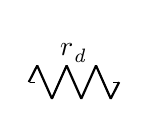
\begin{tikzpicture}[xscale=1,yscale=0.8]
      \draw (0,0)
      to [R=$r_{\mathit{d}}$] (1,0);
    \end{tikzpicture}
  }, of value $r_{\mathit{d}} = \frac{n\kbt}{q(I_{\mathit{D}}+I_{\mathit{S}})}$.

  \coolsection{Second order effects}
  \begin{description}
  \item[Resistive effects] P,N zones show resistive effects, most
    notable at high $I$.
  \item[Avalanche breakdown] For high reverse bias, the big
    $\mathbf{E}$ can accelerate electrons enough to ionize other
    electrons in a chain reaction, generating huge currents.
  \item[Generation-recombination] In inverse bias, generation effects
    (which are predominant) make $I$ be higher than expected. In
    forward bias, recombination effects (dominant,
    $R∼n_\mathit{i}∼\mathrm{e}^{qV/\kbt}$) make current be lower than
    expected. This effects are modeled with $n$, the \textit{ideality
      factor}:
    \begin{equation*}
      I ∼ I_0 \left( \mathrm{e}^{qV/n\kbt}-1 \right)
    \end{equation*}
  \item[High level of injection] Low level of injection is no longer
    the case for high $I$, where $I ∼ e^{qV/2\kbt}$.
  \end{description}

\end{multicols}





\newpage


\begin{tabular}{lr}
  \parbox{0.3\textwidth}
  {
  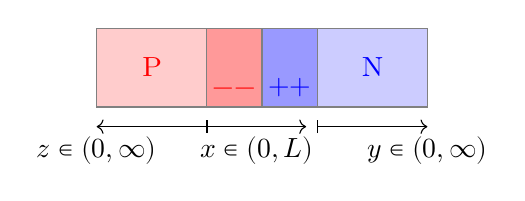
\begin{tikzpicture}[xscale=0.7, yscale=1]
    % Axis and such
    \draw[|->] (1,0) -- (3,0)
    node[at end, below] {$y∊(0,∞)$};
    \draw[|->] (-1,0) -- (-3,0)
    node[at end, below] {$z∊(0,∞)$};
    \draw[|->] (-1,0) -- (0.8,0)
    node[below,midway] {$x∊(0,L)$};
    % Zones
    \draw[thin, gray,fill=red!20!white] (-3,0.25) rectangle
    (-1,1.25); % P
    \draw[thin, gray,fill=red!40!white] (-1,0.25) rectangle
    (0,1.25); % transition P
    \draw[thin, gray,fill=blue!40!white] (0,0.25) rectangle
    (1,1.25); % transition N
    \draw[thin, gray,fill=blue!20!white] (1,0.25) rectangle
    (3,1.25); % N
    % Labels
    \node[below,red] at (-2,1) {\textsc{P}};
    \node[below,blue] at (+2,1) {\textsc{N}};
    \node[above,red] at (-0.5,0.27) {$- -$};
    \node[above,blue] at (+0.5,0.25) {$+ +$};
  \end{tikzpicture}
  }
  \qquad
  \qquad
  \parbox{0.5\textwidth}
  {
  \begin{flushright}
    \textsc{\Huge Solving a Diode}

    \textit{``Because I didn't had anything better to do''}
  \end{flushright}
  }
\end{tabular}

\vspace{0.5cm}

\begin{multicols}{2}

  \coolsection{Transition zone}
  Drift must counteract drag. Using e.g. electrons:
  \begin{equation*}
    \begin{split}
      {\eval{\mathbf{J}_{\mathit{n}}}_\text{drag}}
      =
      qnμ_{\mathit{n}} E_{\mathit{x}} &= -qD_{\mathit{n}} ∇ n
      =
      -{\eval{\mathbf{J}_{\mathit{n}}}_\text{drift}}\\
      -qn \left(\frac{q}{\kbt} \right) \dv{}{x}V &= -qD_{\mathit{n}} \dv{}{x} n
      \\
      \frac{q}{\kbt} \dd{V} &≃ \frac{\dd{n}}{n} \\
      n(x_2) &≃ n(x_1) \mathrm{e}^{\frac{q}{\kbt} (V_2 - V_1)}
    \end{split}
  \end{equation*}
  With $x_2 = x,x_1 = 0$ we obtain
  \begin{align*}
    n(x) &≃ n(0) \mathrm{e}^{qΦ/\kbt} \\
    p(x) &≃ p(0) \mathrm{e}^{-qΦ/\kbt}
  \end{align*}
  With an external potential $V$,
  $
    \underbrace{n(L)}_{≃N_{\mathit{D}}} = n(0) \mathrm{e}^{\frac{q}{\kbt} (Φ_{\mathit{B}} - V)}
    $
    and we end with
    \begin{align*}
      n(0) &= N_{\mathit{D}} \mathrm{e}^{ \frac{q}{\kbt}Φ_{\mathit{B}}}\mathrm{e}^{\frac{q}{\kbt}V} = n_{\mathit{p0}}\cdot  \mathrm{e}^{qV/\kbt}\\
      p(L) &= N_{\mathit{A}} \mathrm{e}^{-\frac{q}{\kbt}Φ_{\mathit{B}}}\mathrm{e}^{\frac{q}{\kbt}V} = p_{\mathit{n0}} \cdot \mathrm{e}^{qV/\kbt}
    \end{align*}

    $Φ_{\mathit{B}}$, the \emph{junction potencial}, can be found using
    $V=0,n(0)=\frac{n_{\mathit{i}}^2}{N_{\mathit{A}}}$ in $\underbrace{n(L)}_{N_{\mathit{D}}}=n(0)
    \mathrm{e}^{qΦ/\kbt}$ as
    \begin{equation*}
      Φ_{\mathit{B}} = \frac{\kbt}{q} \log \frac{N_{\mathit{A}} N_{\mathit{D}}}{n_{\mathit{i}}^2}
    \end{equation*}

    One can solve $Φ(x)$ via Poisson's equation, using that the
    charges in the region are $-qN_\mathit{A}$ and $qN_\mathit{D}$.
    The boundary conditions are $Φ(0)=0$ and $Φ(L)=Φ_B$.
    \begin{equation*}
      Φ(x) =
      \begin{cases}
        \frac{qN_\mathit{A}}{2ε}x^2 &, x∊(0,\ell_p)\\
        \frac{qN_\mathit{D}}{2ε}(x-L)^2 &, x∊(\ell_p,L)
      \end{cases}
    \end{equation*}

    Continuity of the potential gives the value of $L$ as a function
    of $Φ_\mathit{B}$, continuity of $\mathbf{E}$ gives
    $N_\mathit{D}\ell_n = N_\mathit{A}\ell_p$.

  \coolsection{P side}
  The minoritary carriers are electrons. The minoritary carriers move
  mainly through diffusion:
  \begin{equation*}
    \mathbf{J}_{\mathit{p}} ≃ \eval{\mathbf{J}_{\mathit{p}}}_\text{drift} = q D_{\mathit{n}} ∇_{\mathit{n}}
  \end{equation*}
  Use the continuity equation in stationary state:
  \begin{equation*}
    \begin{split}
      \cancelto{0}{\dot{n'}_{\mathit{p}}} &= \frac{1}{q} \pdv{}{z}\mathbf{J}_{\mathit{p}} +
      \cancelto{0}{G_{\mathit{n}}} - \frac{n'_{\mathit{p}}}{τ_{\mathit{n}}}\\
      &= D_{\mathit{n}} \pdv[2]{}{z} n'_{\mathit{p}} - \frac{n'_{\mathit{p}}}{τ_{\mathit{n}}}
    \end{split}
  \end{equation*}
  So $\pdv[2]{n'_{\mathit{p}}}{z} = \frac{n'_{\mathit{p}}}{L^2_{\mathit{n}}}$ with $L^2_{\mathit{n}} = τ_{\mathit{n}}D_{\mathit{n}}$ the
  \emph{diffusion length}, with solution $A \mathrm{e}^{-z/L_{\mathit{n}}} + B \mathrm{e}^{z/L_{\mathit{n}}}$.

  Boundary conditions are:
  \begin{itemize}
  \item $n'_{\mathit{p}} (∞) = 0 \ \rightarrow \ B=0$
  \item $n'_{\mathit{p}}(0) = n_{\mathit{p0}} \mathrm{e}^{qV/\kbt} - n_{\mathit{p0}}$
  \end{itemize}

  We obtain:
  \begin{equation*}
    \boxed{
      n'_{\mathit{p}}(z) = n_{\mathit{p0}} \left( \mathrm{e}^{qV/\kbt} -1 \right) \mathrm{e}^{-z/L_{\mathit{n}}}
    }
  \end{equation*}

  \coolsection{N side}
  Identical. We obtain:
  \begin{equation*}
    \boxed{
      p'_{\mathit{n}}(y) = p_{\mathit{n0}} \left( \mathrm{e}^{qV/\kbt} -1 \right) \mathrm{e}^{-y/L_{\mathit{p}}}
    }
  \end{equation*}

  \coolsection{Current}
  One can show with Gauss' law that $\mathbf{J} \neq f(x)$. Assuming
  no generation-recombination effects in the transition zone (very
  thin) one can write for the transition zone
  $ \mathbf{J}_{\mathit{p}} (x) = \mathbf{J}_{\mathit{p}}(L) $ and $ \mathbf{J}_{\mathit{n}} (x) =
  \mathbf{J}_{\mathit{n}}(0) $.

  We sum minority carriers drift currents in the transition zone
  since both are known. Care must be taken because $\hat{z}$ points
  in the reverse direction from the other axis.
  \begin{equation*}
    \begin{split}
      \mathbf{J}\hat{x} &= \mathbf{J}_{\mathit{p}}(y)\hat{x} - \mathbf{J}_{\mathit{p}}(z)\hat{x} \\
      &= \eval{\left( -qD_{\mathit{p}} \pdv{}{y} p'_{\mathit{n}}(y) \right)}_0 - \eval{\left( q D_{\mathit{n}}
        \pdv{}{z} n'_{\mathit{p}}(z) \right)}_0\\
    &= q \left( \mathrm{e}^{qV/\kbt} -1 \right) \left[ \frac{D_{\mathit{p}} p_{\mathit{n0}}}{L_{\mathit{p}}} +
      \frac{D_{\mathit{n}} n_{\mathit{p0}}}{L_{\mathit{n}}}\right]
    \end{split}
  \end{equation*}

  Define $I$ as going from P to N:
  \begin{equation*}
      I = \int \mathbf{J} \dd{\mathbf{S}} =
      \underbrace{
        qS\left[ \frac{D_{\mathit{p}} p_{\mathit{n0}}}{L_{\mathit{p}}} +
      \frac{D_{\mathit{n}} n_{\mathit{p0}}}{L_{\mathit{n}}}\right]
  }_{I_{\mathit{S}}} \left( \mathrm{e}^{\frac{qV}{\kbt}}-1 \right)
  \end{equation*}

  If a non zero rate of generation-recombination is assumed in the
  transition zone, one can approximate
  \begin{equation*}
    \boxed{
      I =
      I_{\mathit{S}} \left[ \exp(\frac{qV}{n\kbt})-1 \right]
    }
  \end{equation*}
  for $n∊(1,2)$.


\end{multicols}


\newpage


\begin{center}
\textsc{\Huge MOS transistor}

\textit{``Twice the diodes, twice as better''}
\end{center}

\vspace{0.5cm}

    \tikzstyle{n}=[fill=blue!40!white]
    \tikzstyle{p}=[fill=red!60!white]
    \tikzstyle{channel}=[fill=red!40!white]
    \tikzstyle{metal}=[fill=black!60!white]
    \tikzstyle{insulator}=[fill=orange!60!white]

    \begin{center}
      \begin{tikzpicture}[>=stealth,xscale=0.8]
        % Styles
        % Draw elements
        \draw[n] (0,0) rectangle (5,-1.5);
        \fill[channel] (1.5,0) -- (3.5,0) -- (3.5,-0.25) -- (1.5,-0.4);
        \draw[p] (0.5,0) rectangle (1.5,-0.5);
        \draw[p] (3.5,0) rectangle (4.5,-0.5);
        \draw[insulator] (1.5,0) rectangle (3.5,0.15);
        \draw[metal] (1.5,0.15) rectangle (3.5,0.30);
        \draw[metal] (1.5,-1.5) rectangle (3.5,-1.65);
        \draw[metal] (0.75,0) rectangle (1.25,0.15);
        \draw[metal] (3.75,0) rectangle (4.25,0.15);
        % Draw labels
        \node[above right,color=blue] at (0,-1.5) {$n^+$};
        \node[] at (1,-0.25) {$p^+$};
        \node[] at (4,-0.25) {$p^+$};
        \draw[|-|] (1.5,-0.8) -- (3.5,-0.8) node[midway, fill=blue!40!white] {$L$};
        % Draw two diodes
        \ctikzset{bipoles/length=5mm}
        \draw (1.25,-0.40) to[D*] (1.25,-0.75);
        \draw (3.75,-0.40) to[D*] (3.75,-0.75);
        % Draw wires
        \draw (1,0.15) to[short] (1,0.5) to[short,-o] (0,0.5) node[left] {$V_{\mathit{S}}$};
        \draw (4,0.15) to[short] (4,0.5) to[short,-o,i<=$I_{\mathit{D}}$] (5,0.5) node[right] {$V_{\mathit{D}}$};
        \draw (2.5,0.30) to[short,-o] (2.5,0.6) node[right] {$V_{\mathit{G}}$};
        \draw (2.5,-1.65) to[short,-o] (2.5,-2) node[right] {$V_{\mathit{B}}$};
        % Draw axis markings
        \draw[->] (1.5,0) -- (2.5,0) node [below] {$\hat{y}$};
        \draw[->] (1.5,0) -- (1.5,-0.5) node [right] {$\hat{x}$};
        \draw[fill=black] (1.5,0) circle (0.1);
      \end{tikzpicture}
      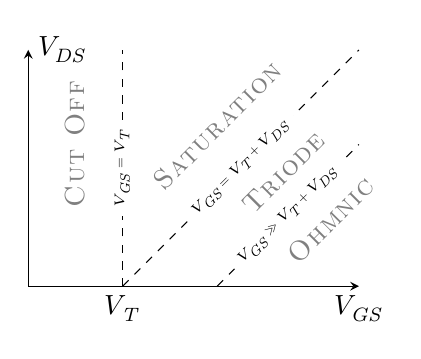
\begin{tikzpicture}[>=stealth,scale=1.2]
        % Axis
        \draw[->] (0,0) -- (3.5,0) node [at end,below] {$V_{\mathit{GS}}$};
        \draw[->] (0,0) -- (0,2.5) node [at end,right] {$V_{\mathit{DS}}$};
        % Region separators, labels
        \draw[dashed] (1,0) -- (1,2.5)
        node[midway,sloped,fill=white] {\tiny $V_{\mathit{GS}}=V_{\mathit{T}}$}
        node[at start, below] {$V_{\mathit{T}}$};
        \draw[dashed] (1,0) -- (3.5,2.5)
        node[midway,sloped,fill=white] {\tiny $V_{\mathit{GS}}=V_{\mathit{T}}+V_{\mathit{DS}}$};
        \draw[dashed] (2,0) -- (3.5,1.5)
        node[midway,sloped,fill=white] {\tiny $V_{\mathit{GS}} ≫ V_{\mathit{T}}+V_{\mathit{DS}}$};
        % Regions
        \node[rotate=90,gray] at (0.5,1.5) {\textsc{Cut Off}};
        \node[rotate=45,gray] at (2,1.7) {\textsc{Saturation}};
        \node[rotate=45,gray] at (2.7,1.2) {\textsc{Triode}};
        \node[rotate=45,gray] at (3.2,0.7) {\textsc{Ohmnic}};
      \end{tikzpicture}
      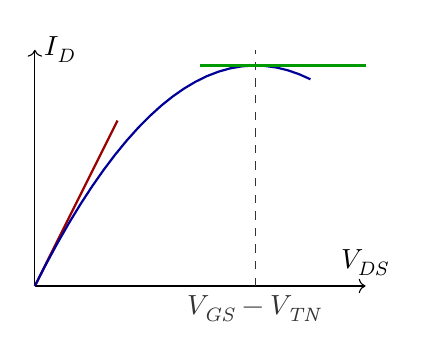
\begin{tikzpicture}[xscale=0.7]
        \draw[->] (0,0) -- (6,0) node[above, at end] {$V_{\mathit{DS}}$};
        \draw[->] (0,0) -- (0,3) node[right, at end] {$I_{\mathit{D}}$};
        \draw[dashed,black!80!white] (4,0) -- (4,3) node[below, at
        start] {$V_{\mathit{GS}}-V_{\mathit{TN}}$}; \draw[thick,red!60!black]
        plot[domain=0:1.5] (\x,{0.35*4*\x}); \draw[thick,blue!60!black]
        plot[domain=0:5] (\x,{0.35*(4*\x-\x*\x/2)});
        \draw[thick,green!60!black] plot[domain=3:6] (\x,{0.35/2*4*4});
      \end{tikzpicture}
    \end{center}

    \hrule

\begin{multicols}{2}

  \coolsection{MOS capacitor (P)}
  \begin{center}
    \begin{tikzpicture}[>=stealth]
      \draw[metal] (0,0) rectangle (1,-0.25);
      \draw[insulator] (0,-0.25) rectangle (1,-1);
      \draw[p] (0,-1) rectangle (1,-2.5);
      \fill[red!70!white] (0,-1) rectangle (1,-1.5)
      node [midway,black] {\tiny $qp$};
      \draw (0.5,0) to[short,-o] (0.5,0.5) node[right] {\tiny $V_{\mathit{G}}$};
      \node[below] at (0.5,-2.5) {\tiny $V_{\mathit{G}}<V_{\mathit{FB}}$};
      \draw (0,0) rectangle (1,-2.5);
    \end{tikzpicture}
    \begin{tikzpicture}[>=stealth]
      \draw[metal] (0,0) rectangle (1,-0.25);
      \draw[insulator] (0,-0.25) rectangle (1,-1);
      \draw[p] (0,-1) rectangle (1,-2.5);
      \fill[blue!20!white] (0,-1) rectangle (1,-1.5)
      node [midway,black] {\tiny $-qN_{\! A}$};
      \draw (0.5,0) to[short,-o] (0.5,0.5) node[right] {\tiny $V_{\mathit{G}}$};
      \node[below] at (0.5,-2.5) {\tiny $V_{\mathit{G}}∊(V_{\mathit{FB}},V_{\mathit{T}})$};
      \draw (0,0) rectangle (1,-2.5);
    \end{tikzpicture}
    \begin{tikzpicture}[>=stealth]
      \draw[metal] (0,0) rectangle (1,-0.25);
      \draw[insulator] (0,-0.25) rectangle (1,-1);
      \draw[p] (0,-1) rectangle (1,-2.5);
      \fill[blue!40!white] (0,-1) rectangle (1,-1.5)
      node [midway,black] {\tiny $-qn$};
      \fill[blue!20!white] (0,-1.5) rectangle (1,-2)
      node [midway,black] {\tiny $-qN_{\! A}$};
      \draw (0.5,0) to[short,-o] (0.5,0.5) node[right] {\tiny $V_{\mathit{G}}$};
      \draw (1,-1.25) to[short,-o] (1.5,-1.25) node[above] {\tiny $V_1$};
      \node[below] at (0.5,-2.5) {\tiny $V_{\mathit{G}}>V_{\mathit{T}}$};
      \draw (0,0) rectangle (1,-2.5);
    \end{tikzpicture}
  \end{center}
  \begin{itemize}
  \item Accumulation in reverse bias.
  \item Depletion, ${N_{\mathit{A}} > p > n}$.
  \item Weak inversion , $N_{\mathit{A}} > n > p$.
  \item Strong inversion, $n>N_{\mathit{A}} > p$.
  \end{itemize}

  Charge in the strong inversion channel:
  \begin{equation*}
    \int qn \dd{x} = -Q = C_0 (V_{\mathit{G}} -V_1 - V_{\mathit{TN}})
  \end{equation*}
  With $V_{\mathit{B}}=0$,
  \begin{equation*}
    V_{\mathit{TN0}} = 2Φ_0 + V_{\mathit{FB}} + γ \sqrt{2Φ_0}
  \end{equation*}

  Each $y$ of the MOS channel is a MOS capacitor!

  \coolsection{Regions}
  \begin{description}

  \item[Cut off]
    \begin{tikzpicture}[>=stealth,scale=0.3]
      \draw[n] (0,0) rectangle (5,-0.7);
      %\fill[channel] (1.5,0) -- (3.5,0) -- (3.5,-0.25) -- (1.5,-0.4);
      \draw[p] (0.5,0) rectangle (1.5,-0.5);
      \draw[p] (3.5,0) rectangle (4.5,-0.5);
    \end{tikzpicture}
    $V_{\mathit{GS}}<V_{\mathit{TN}}$ implies no channel at all.

  \item[Ohmnic]
    \begin{tikzpicture}[>=stealth,scale=0.3]
      \draw[n] (0,0) rectangle (5,-0.7);
      %\fill[p] (1.5,0) -- (3.5,0) -- (3.5,-0.25) -- (1.5,-0.4);
      \fill[p] (1.5,0) -- (3.5,0) -- (3.5,-0.50) -- (1.5,-0.50);
      \draw[p] (0.5,0) rectangle (1.5,-0.5);
      \draw[p] (3.5,0) rectangle (4.5,-0.5);
    \end{tikzpicture}
    Homogeneous channel.
    $V_{\mathit{GS}}>V_{\mathit{TN}}$ and $V_{\mathit{GS}}-V_{\mathit{TN}}\gg V_{\mathit{DS}}$,
    so
    \begin{equation*}
      \int_{\mathrlap{\text{channel}}} q n \dd{x} \simeq C_0
      [V_{\mathit{GS}}-V_{\mathit{TN}}+\cancelto{∼0}{V(y)}]
    \end{equation*}

  \item[Triode]
    \begin{tikzpicture}[>=stealth,scale=0.3]
      \draw[n] (0,0) rectangle (5,-0.7);
      \fill[p] (1.5,0) -- (3.5,0) -- (3.5,-0.1) -- (1.5,-0.5);
      \draw[p] (0.5,0) rectangle (1.5,-0.5);
      \draw[p] (3.5,0) rectangle (4.5,-0.5);
    \end{tikzpicture}
    The channel is not homogeneous.
    Impose that there is still channel $∀y$:
    \begin{align*}
      \eval{\int qn \dd{x}}_{y=0} \geq 0 \ &\rightarrow \ V_{\mathit{GS}} \geq V_{\mathit{TN}}\\
      \eval{\int qn \dd{x}}_{y=L} \geq 0 \ &\rightarrow \ V_{\mathit{GS}}-V_{\mathit{TN}}
                                          \geq V_{\mathit{DS}}
    \end{align*}

  \item[Saturation / active]
    \begin{tikzpicture}[>=stealth,scale=0.3]
      \draw[n] (0,0) rectangle (5,-0.7);
      \fill[p] (1.5,0) -- (2.5,0) -- (2.5,-0.1) -- (1.5,-0.5);
      \draw[p] (0.5,0) rectangle (1.5,-0.5);
      \draw[p] (3.5,0) rectangle (4.5,-0.5);
    \end{tikzpicture}
    There are values of $y$ without channel.
    \begin{align*}
      \eval{\int qn \dd{x}}_{y=0} \geq 0 \ &\rightarrow \ V_{\mathit{GS}} \geq V_{\mathit{TN}}\\
      \eval{\int qn \dd{x}}_{y=L} \leq 0 \ &\rightarrow \ V_{\mathit{GS}}-V_{\mathit{TN}}
                                          \leq V_{\mathit{DS}}
    \end{align*}

    Starts when $V(L)=V_{\mathit{GS}}-V_{\mathit{TN}}≔V_\text{sat}$. Despite not being
    channel in some $y$, the electric field is strong and conduction
    continues, the depleted region conduces without problem.
  \end{description}

  For a PMOS they are the same, but with the inequalities reversed
  ($C_0 \to -C_0$).

  \coolsection{Characteristic equation}
  \vspace{-7mm}
  \begin{align*}
    I_{\mathit{D}} &= β (V_{\mathit{GS}}-V_{\mathit{TN}})V_{\mathit{DS}}
          \tag{\textcolor{red!60!black}{Ohmnic}}\\
    I_{\mathit{D}} &= β \left[ (V_{\mathit{GS}}-V_{\mathit{TN}})V_{\mathit{DS}} - \frac{V_{\mathit{DS}}^2}{2} \right]
          \tag{\textcolor{blue!60!black}{Triode}}\\
    I_{\mathit{D}} &= \frac{β}{2}(V_{\mathit{GS}}-V_{\mathit{TN}})^2
          \tag{\textcolor{green!60!black}{Saturation}}
  \end{align*}

  with $β=C_0μ_{\mathit{n}}\frac{W}{L}$. Everything at 1\textsuperscript{st}
  order of aproximation. The region depends on the \textit{operation
    point}, given by $(I_{\mathit{DS}},V_{\mathit{DS}})$. Valid for
  both PMOS and NMOS.

  \coolsection{AC model \textcolor{black!60!white}{(active zone)}}
  \begin{center}
    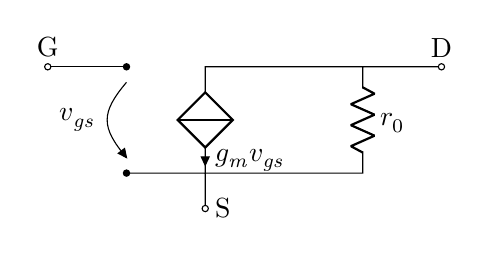
\begin{tikzpicture}[yscale=0.9]
      \ctikzset{bipoles/length=1cm}
      % G
      \draw (0,0) node [above] {G}
      to[short,o-*] (1,0)
      ;
      % Vgs
      \draw (1,0)
      to[open,v=$v_{\mathit{gs}}$] (1,-1.5)
      ;
      % D
      \draw (5,0) node [above] {D}
      to[short,o-] (2,0)
      to[cI=$g_{\mathit{m}}v_{\mathit{gs}}$] (2,-1.5)
      to[short] (4,-1.5)
      to[R,l_=$r_0$] (4,0)
      ;
      % Ground
      \draw (1,-1.5)
      to[short,*-] (1,-1.5)
      to[short] (2,-1.5)
      to[short,-o] (2,-2.0)
      node[right] {S}
      ;
    \end{tikzpicture}
  \end{center}
  where PMOS have
  \raisebox{-1mm}{
    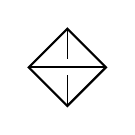
\begin{tikzpicture}
      \draw (0,0) to[cI] (0,0.2);
    \end{tikzpicture}
    }
    instead (or, alternatively, changes $v_\textit{gs} \to
    v_\textit{sg}$) and
  \begin{equation*}
    g_{\mathit{m}} = \frac{2I_{\mathit{DS}}}{\abs{V_{\mathit{GS}}-V_{\mathit{T}}}}
    \qquad
    r_0 = \left(
      \frac{
        λI_{\mathit{DS}}
      }{
        \cancel{1+λV_{\mathit{DS}}}
      } \right)^{-1}
  \end{equation*}
  Also, $g_{\mathit{m}} = β(V_{\mathit{GS}}-V_{\mathit{T}})=
  \sqrt{2βI_{\mathit{DS}}}$ in the saturation region.


\end{multicols}


\newpage



\begin{tabular}{lr}
  \parbox{0.3\textwidth}
  {
  \begin{tikzpicture}[xscale=2.0, yscale=1.5]
    % Axis and such
    \draw[|->,>=stealth] (0,-0.5) -- (2.5,-0.5)
    node[at start, below] {$x∊(0,∞)$};
    \draw[|-|] (1,-0.5) -- (1.5,-0.5)
    node[at start, below] {$t_\mathit{ox}$}
    ;
    \draw[|-|] (1.5,-0.5) -- (2,-0.5)
    node[at start, below] {$t_\mathit{ox}\!\!+\!a$}
    node[at end, below] {$\qquad t_\mathit{ox}\!\!+\!a\!\!+\!\!L$}
    ;
    % Zones
    \draw[insulator] (0.0,0) rectangle (1,1);
    \draw[metal] (0,0) rectangle (0.05,1);
    \draw[p] (1,0) rectangle (2.5,1);
    \fill[blue!40!white] (1,0) rectangle (1.5,1)
    node [midway,black] {$-qn$};
    \fill[blue!20!white] (1.5,0) rectangle (2,1)
    node [midway,black] {$-qN_{\! A}$};
    \draw (0,0.5) to[short,-o] (-0.5,0.5) node[above] {$V_{\mathit{G}}$};
    \draw (2.5,0.5) to[short,-o] (3,0.5) node[above] {$V_{\mathit{B}}$};
    \draw (1,1) to[short,-o] (1,1.5) node[right] {$V_\mathit{CB'}$};
    \draw[metal] (2.45,0) rectangle (2.5,1);
    \draw (0,0) rectangle (2.5,1);
  \end{tikzpicture}
  }
  \qquad
  \qquad
  \qquad
  \parbox{0.5\textwidth}
  {
  \begin{flushright}
    \textsc{\Huge Solving a MOS capacitor}

    \textit{``Fun AF!''}
  \end{flushright}
  }
\end{tabular}

\vspace{0.5cm}

\begin{multicols*}{2}
  \coolsection{Voltages}
  We do KVL from $x=0$ to $x=\infty$:
  \begin{equation*}
    V_G = \underbrace{[ V(0) - V(t_\mathit{ox})  ]}_{V_\mathit{ox}} +
    \underbrace{[V(t_\mathit{ox}) -
    V(\infty)]}_{V_\mathit{CB'}}
    - Φ_\textit{CMP} + V_B
  \end{equation*}
  where $Φ_\textit{CMP}$ is the voltage across the metal contact in
  $V_\mathit{B}$. Reordering terms, we obtain the voltage in the insulator:
  \begin{equation*}
    \boxed{
      V_\mathit{ox} = V_\mathit{G} - V_\mathit{B} + Φ_\mathit{CMP} - V_\mathit{CB'}
    }
  \end{equation*}
\coolsection{Channel charge}
\textsc{In the insulator}, $∇\mathbf{D}=0$ so the displacement is constant and
$\mathbf{E}=-∇V = \frac{D_0}{ε}$.
We obtain a voltage $V_\mathit{ox} = \frac{D_0}{ε} t_\mathit{ox}$
after integrating in $x∈(0,t_\mathit{ox})$. The displacement can be
writen in terms of this voltage $D_0 = \frac{ε}{t_\mathit{ox}}
V_\mathit{ox} = C_0 V_\mathit{ox}$.

\textsc{In the semiconductor}, we have $∇\mathbf{D}=ρ$, so
$\dd{D}\hat{x} = ρ \dd{x} \hat{x}$; let's integrate (why not) that in
$x∈(t_\mathit{ox},\infty)$:
\begin{equation*}
  \begin{split}
    \int_{t_\mathit{ox}}^\infty \hat{x} \mathbf{D} \dd{D} &= \int_0^\infty ρ \dd{x} \\
    \cancelto{0}{D(\infty)} - D(t_\mathit{ox})
    &=
    \int_{t_\mathit{ox}}^{\mathrlap{t_\mathit{ox}+a}} ρ \dd{x}
    +\int_{t_\mathit{ox}+a}^{\mathrlap{t_\mathit{ox}+a+L}} ρ \dd{x}
    +\cancelto{0}{\int_{\mathrlap{{t_\mathit{ox}+a+L}}}^{\infty} ρ \dd{x}}
    \\
     - D(t_\mathit{ox})
    &=
    \underbrace{\int_{\mathrlap{t_\mathit{ox}}}^{\mathrlap{t_\mathit{ox}+a}} -qn
      \dd{x}}_{\text{Str. Inv.}}
    + \underbrace{\int_{\mathrlap{t_\mathit{ox}+a}}^{\mathrlap{t_\mathit{ox}+a+L}}
      -qN_\mathit{A} \dd{x}}_{\text{Weak Inv.}}
    + \underbrace{0}_{\text{P region}}
    \\
  \end{split}
\end{equation*}

So we obtain
\begin{equation*}
  \begin{split}
    \int_{\mathrlap{t_\mathit{ox}}}^{\mathrlap{t_\mathit{ox}+a}} qn
    \dd{x} &= D(t_\mathit{ox}) - qN_\mathit{A} L \\
    &= C_0V(t_\mathit{ox}) - qN_\mathit{A} L \\
    &= C_0 [V_\mathit{G} - V_\mathit{B} + Φ_\mathit{CMP} - V_\mathit{CB'}] - qN_\mathit{A} L \\
    &= C_0 \left[ V_\mathit{G} - V_\mathit{B} + Φ_\mathit{CMP} -
      V_\mathit{CB'} - \frac{qN_\mathit{A}}{C_0} L \right]\\
    &= C_0 \left[ V_\mathit{G} - V_\mathit{B} - V_\mathit{CB'} -
      \left( -Φ_\mathit{CMP}+\frac{qN_\mathit{A}}{C_0} L \right)\right]\\
  \end{split}
\end{equation*}
where  $V(t_\mathit{ox})$ has been
substituted by the monster found in the \textsc{Voltages} section.
Because we added a strong inversion layer in the analysis,
$V_\mathit{CB'}$ must be at least $2Φ_0$ so it forms.

We are interested in an expresion that is a function of
$V_1 = V_\mathit{CB'}  + V_\mathit
{B} + Φ_\mathit{cmp}$, which is basically
the voltage $V_\mathit{CB'}$ refered to $V_\mathit{B}$ taking care of
the metal contact voltage difference. Grouping everything else into a
constant $V_\mathit{TN}$,
\begin{equation*}
  \boxed{
  \int_{\mathrlap{t_\mathit{ox}}}^{\mathrlap{t_\mathit{ox}+a}} qn
  \dd{x} =
  C_0 [ V_\mathit{G} - V_1 - V_\mathit{TN}]
  }
\end{equation*}

\end{multicols*}


\newpage

\begin{center}
\textsc{\Huge BJT transistor}

\textit{``I love the smell of a PN junction in the morning''}
\end{center}

\vspace{0.5cm}

\begin{multicols}{2}

  \begin{center}
  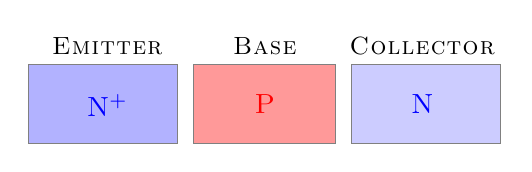
\begin{tikzpicture}
    % Zones
    \draw[thin, gray,fill=blue!30!white] (-3,0.25) rectangle
    (-1.1,1.25); % N⁺
    \draw[thin, gray,fill=red!40!white] (-0.9,0.25) rectangle
    (0.9,1.25); % P
    \draw[thin, gray,fill=blue!20!white] (1.1,0.25) rectangle
    (3,1.25); % N
    % Labels
    \node[below,blue] at (-2,1) {\textsc{N}\textsuperscript{+}};
    \node[below,red] at (+0,1) {\textsc{P}};
    \node[below,blue] at (+2,1) {\textsc{N}};
    % Region labels
    \node[above] at (-2,1.25) {\small \textsc{Emitter}};
    \node[above] at (0,1.25)  {\small \textsc{Base}};
    \node[above] at (2,1.25)  {\small \textsc{Collector}};
  \end{tikzpicture}
  \end{center}
  \begin{center}
    \begin{circuitikz}
      \draw (0,0) node[npn,rotate=-90] (npn) {};
      \draw (npn.E) node[left] {E};
      \draw (npn.B) node[right] {B};
      \draw (npn.C) node[right] {C};
      \draw (3,0) node[pnp,rotate=-90] (pnp) {};
      \draw (pnp.E) node[right] {E};
      \draw (pnp.B) node[right] {B};
      \draw (pnp.C) node[left] {C};
    \end{circuitikz}
  \end{center}
  \coolsection{Inverse biased diode}
  The main idea is to control the saturation current of a diode. We
  model this as a controled generator of $I=I_{\mathit{SC}}$ in series with the
  diode, of current $I=I_{\mathit{S}}$ (saturation current).

  \begin{center}
    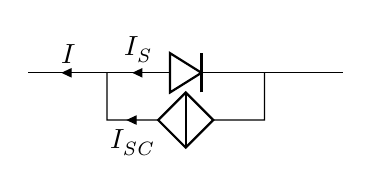
\begin{tikzpicture}[yscale=0.6]
      \ctikzset{bipoles/length=1cm}
      % Diode
      \draw (0,0)
      to[short,i<=$I$] (1,0)
      to[Do,i<=$I_{\mathit{S}}$] (3,0)
      to[short] (4,0)
      ;
      % Source
      \draw (3,0)
      to[short] (3,-1)
      to[cI=$I_{\mathit{SC}}$] (1,-1)
      to[short] (1,0)
      ;
    \end{tikzpicture}
  \end{center}

  \coolsection{Two diode model}
  General model for all work regions.

  \begin{center}
    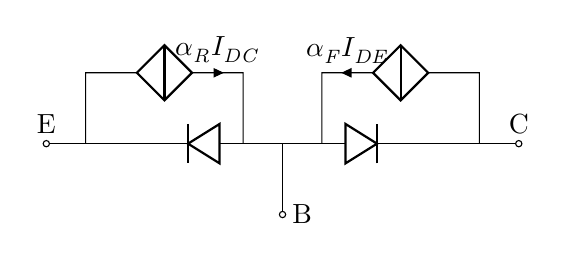
\begin{tikzpicture}[yscale=0.9]
      \ctikzset{bipoles/length=1cm}
      \draw (0,0)
      to[Do] (-2,0)
      to[short,-o] (-3,0) node[above] {E}
      ;
      \draw (0,0)
      to[Do] (2,0)
      to[short,-o] (3,0) node[above] {C}
      ;
      \draw (0,0) to [short,-o] (0,-1) node[right] {B}
      ;
      \draw (-2.5,0)
      to[short] (-2.5,1)
      to[cI=$α_{\mathit{R}} I_{\mathit{DC}}$] (-0.5,1)
      to[short] (-0.5,0)
      ;
      \draw (2.5,0)
      to[short] (2.5,1)
      to[cI_=$α_{\mathit{F}} I_{\mathit{DE}}$] (0.5,1)
      to[short] (0.5,0)
      ;
    \end{tikzpicture}
  \end{center}
  \begin{align*}
    I_{\mathit{E}} &= I_{\mathit{ES}} \vbe - α_{\mathit{R}} I_{\mathit{CS}} \vbc \\
    I_{\mathit{C}} &= α_{\mathit{F}} I_{\mathit{ES}} \vbe - I_{\mathit{CS}} \vbc \\
    I_{\mathit{B}} &= I_{\mathit{E}} - I_{\mathit{C}}
  \end{align*}
  with $α_{\mathit{R}} I_{\mathit{CS}} = α_{\mathit{F}}I_{\mathit{ES}}=I_{\mathit{S}}=qAD_{\mathit{b}} \frac{n_{\mathit{b0}}}{W}$. This
  equations (\textsc{Elbers-Moll equations}) are too complicated for
  direct use, and simplifications are made depending on the work region.

  The relationship of $I_{\mathit{S}}$ with $W$ shows that a small base region
  increases the diode interdependency.

  \coolsection{Region models (NPN)}
  The region depends on the \textit{operation point}, $(I_{\mathit{C}},V_{\mathit{CE}})$.
  \paragraph{Cut}
  Both junctions are inversely polarized, so $\mathrm{e}^{qV/\kbt}∼0$. The only
  current is the diode saturation current, which can be neglected.
  \begin{center}
    \begin{tikzpicture}[scale=0.5]
      \ctikzset{bipoles/length=1cm}
      \draw (0,0) node[above] {B}
      to[short,o-*] (2,0)
      to[open] (4,0)
      to[short,*-o] (6,0) node[above] {C}
      ;
      \draw (3,-2)
      to[short,*-o] (3,-4) node[right] {E}
      ;
    \end{tikzpicture}
  \end{center}

  \paragraph{Saturation}
  Both junctions are forward polarized; the circuit is equivalent to a
  short circuit with the PN junctions voltage drops.
  \begin{center}
    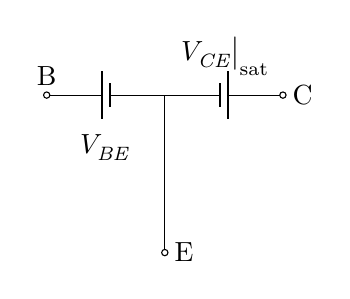
\begin{tikzpicture}[scale=0.5]
      \ctikzset{bipoles/length=1cm}
      \draw (0,0) node[above] {B}
      to[battery1,l_=$V_{\mathit{BE}}$,o-] (3,0);
      \draw (3,-4) node[right] {E}
      to[short,o-] (3,0)
      ;
      \draw (6,0) node[right] {C}
      to[battery1,l_=$\eval{V_{\mathit{CE}}}_\text{sat}$,o-] (3,0)
      ;
    \end{tikzpicture}
  \end{center}

  \paragraph{Active}
  Base-emitter junction forward biased, but base-collector junction
  reverse biased. This is the main region of the transistor, in which
  it behaves like an amplifier.
  \begin{center}
    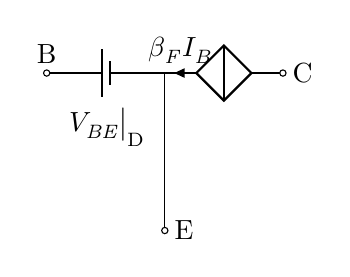
\begin{tikzpicture}[scale=0.5]
      \ctikzset{bipoles/length=1cm}
      \draw (0,0) node[above] {B}
      to[battery1,l_=$\eval{V_{\mathit{BE}}}_\text{D}$,o-] (3,0);
      \draw (3,-4) node[right] {E}
      to[short,o-] (3,-1)
      to[short] (3,0)
      ;
      \draw (6,0) node[right] {C}
      to[cI_=$β_{\mathit{F}} I_{\mathit{B}}$,o-] (3,0)
      ;
    \end{tikzpicture}
  \end{center}
  where $β_{\mathit{F}}= \frac{α_{\mathit{F}}}{α_{\mathit{F}}-1}$.

\paragraph{Active inverse}
Is identical to the \emph{active} zone, but the emitter and the
collector switch roles. Is not very used because of the BJT being
optimized for forward operation.
The emitter is more doped than the collector for this exact thing.

PNP transistors are identical but defining $I_E,I_C$ in the opposite
sense (from emitter to collector) and reversing the current generator.

\coolsection{AC model}
\begin{center}
  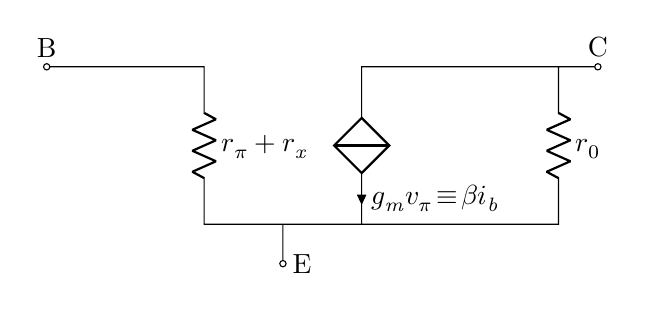
\begin{tikzpicture}
      \ctikzset{bipoles/length=1cm}
      \draw (0,0) node[above] {B}
      to[short,o-] (2,0)
      to[R=$r_π+r_{\mathit{x}}$] (2,-2)
      to[short] (3,-2)
      to[short,-o] (3,-2.5) node[right] {E}
      to[short] (3,-2)
      to[short] (4,-2)
      to[short] (6.5,-2)
      to[R,l_=$r_0$] (6.5,0)
      to[short,-o] (7,0) node[above] {C}
      to[short] (4,0)
      to[cI=$ g_{\mathit{m}} v_π\! \equiv\! βi_{\mathit{b}} $] (4,-2)
      ;
  \end{tikzpicture}
\end{center}

where $r_{\mathit{x}}$ is the resistance of the base terminal. For a PNP, the
model is exactly the same but $I_{\mathit{B}}$, $I_{\mathit{E}}$ and $I_{\mathit{C}}$ are defined in
the opposite sense (and the current generator is reversed). The parameters are given by:
\begin{equation*}
  \frac{q}{\kbt} I_{\mathit{C}} = g_{\mathit{m}} \qquad \frac{I_{\mathit{C}}}{V_{\mathit{A}} + V_{\mathit{CE}}} =
  \frac{1}{r_0} \qquad \frac{g_{\mathit{m}} }{β_0} = \frac{1}{r_π}
\end{equation*}

Sometimes, the \textit{hybrid model} is used, and $h_{\mathit{fe}}\equiv
\beta$ and $h_{\mathit{ie}}\equiv r_\pi + r_{\mathit{x}}$ are given.

\end{multicols}

\newpage


\begin{tabular}{lr}
  \parbox{0.3\textwidth}
  {
  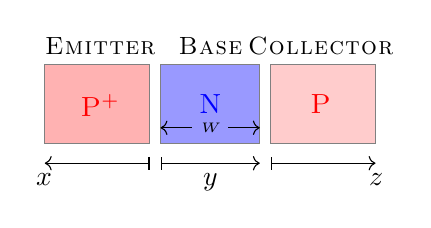
\begin{tikzpicture}[xscale=0.7, yscale=1]
    % Axis and such
    \draw[|->] (-1.1,0) -- (-3,0)
    node[at end, below] {$x$};
    \draw[|->] (-0.9,0) -- (0.9,0)
    node[below,midway] {$y$};
    \draw[|->] (1.1,0) -- (3,0)
    node[at end, below] {$z$};
    % Zones
    \draw[thin, gray,fill=red!30!white] (-3,0.25) rectangle
    (-1.1,1.25); % P⁺
    \draw[thin, gray,fill=blue!40!white] (-0.9,0.25) rectangle
    (0.9,1.25); % N
    \draw[thin, gray,fill=red!20!white] (1.1,0.25) rectangle
    (3,1.25); % P
    % Labels
    \node[below,red] at (-2,1) {\textsc{P}\textsuperscript{+}};
    \node[below,blue] at (+0,1) {\textsc{N}};
    \node[below,red] at (+2,1) {\textsc{P}};
    % width
    \draw[<->] (-0.9,0.45) -- (0.9,0.45)
    node[midway,fill=blue!40!white] {\tiny $W$};
    % Region labels
    \node[above] at (-2,1.25) {\small \textsc{Emitter}};
    \node[above] at (0,1.25)  {\small \textsc{Base}};
    \node[above] at (2,1.25)  {\small \textsc{Collector}};
  \end{tikzpicture}
  }
  \qquad
  \qquad
  \parbox{0.5\textwidth}
  {
  \begin{flushright}
    \textsc{\Huge Solving a BJT}

    \textit{``You never have enough diodes''}
  \end{flushright}
  }
\end{tabular}

\vspace{0.5cm}

\begin{multicols}{2}

  \coolsection{Carrier concentrations}
  The continuity equation is the same for all the regions,
  with solution of the style $A \mathrm{e}^{ζ/L} + B \mathrm{e}^{ζ/L}$.

  \paragraph{Emitter}
  Solve $
    \dv{}{x^2}p_{\mathit{e}}' = p_{\mathit{e}}'/L_{\mathit{e}}^2
    $ with
  boundary conditions:
  $
  p_{\mathit{e}}'(0) = p_{\mathit{e0}} \vbe
  $
  and
  $
    p_{\mathit{e}}'(∞) = 0
    $.
  Solution:
  \begin{equation*}
      p_{\mathit{e}}'(x) = p_{\mathit{e0}} \vbe \mathrm{e}^{-x/L_{\mathit{e}}}
  \end{equation*}

  \paragraph{Collector}
  Exactly the same.
  \begin{equation*}
      p_{\mathit{c}}'(z) = p_{\mathit{c0}} \vbc \mathrm{e}^{-z/L_{\mathit{e}}}
  \end{equation*}

  \paragraph{Base}
  The boundary conditions are a bit more difficult, so the ending
  expresion is more complicated.
  \begin{align*}
    n_{\mathit{b}}'(0) &= n_{\mathit{b0}} \vbe \\
    n_{\mathit{b}}'(W) &= n_{\mathit{b0}} \vbc
  \end{align*}

  At the end of the day, we obtain
  \begin{equation*}
    \begin{split}
      n_{\mathit{b}}'(y) = \frac{n_{\mathit{b0}}}{\sinh(W/L_{\mathit{b}})} \Big[
      &\vbe \sinh \frac{W-y}{L_{\mathit{b}}} \\
      + &\vbc \sinh \frac{y}{L_{\mathit{b}}}
      \Big]
    \end{split}
  \end{equation*}

  We can assume than generation-recombination rate is small; $n_{\mathit{b}}' /
  L_{\mathit{b}}^2 \sim 0$ in the differential equation or $W≪L_{\mathit{b}}$ in the full
  expression. With this approximation, we obtain:
  \begin{equation*}
    \begin{split}
      n_{\mathit{b}}'(y) &= n_{b_0} \vbe \\
      &- n_{\mathit{b0}} \left( \mathrm{e}^{qV_{\mathit{BE}}/\kbt}
        - \mathrm{e}^{qV_{\mathit{BC}}/\kbt} \right) \frac{y}{W}
  \end{split}
  \end{equation*}
  in a first order aproximation, $\sinh x = x + \order{x^2}$. We
  obtain something proportional to $y$.

  \coolsection{Current densities}
  For the minoritary carriers, they are just the drift currents
  ($∼ qD\nabla n$). We evaluate the emitter and collector currents in
  the boundary of the transition zone:
  \begin{align*}
    \mathbf{J}_{\mathit{pe}} (0) &= q \frac{D_{\mathit{e}}p_{\mathit{e0}}}{L_{\mathit{e}}} \vbe \hat{x} \\
    \mathbf{J}_{\mathit{pc}} (0) &= -q \frac{D_{\mathit{c}}p_{\mathit{c0}}}{L_{\mathit{c}}} \vbc \hat{y}
  \end{align*}
  For the base current we derivate the full hiperbolic expression, and
  substitute $\cosh ε ∼ 1$:
  \begin{equation*}
    \begin{split}
      \mathbf{J}_{\mathit{nb}} (y) = -q \frac{D_{\mathit{b}}n_{\mathit{b0}}}{W} \Big[ &\vbe\\ - &\vbc
      \Big] \hat{z}
    \end{split}
  \end{equation*}

  \coolsection{Intensities}
  They are independent of the coordinate, so we do the same trick as
  in the diode and compute them in the transition zone to be able to
  sum both carriers.

  Beware the sign changes due to $\hat{x}$ being in the opposite
  direction from $\hat{y},\hat{z}$.
  \paragraph{Emitter}
  \begin{equation*}
    \begin{split}
      \mathbf{J}_{\mathit{E}} &≃ \mathbf{J}_{\mathit{n}} (y=0) + \mathbf{J}_{\mathit{p}} (x=0) \\
      &= -q D_{\mathit{b}} \frac{n_{\mathit{b0}}}{W} \left[ \vbe - \vbc \right] (-\hat{x})
      \\
      &+ q D_{\mathit{e}} \frac{p_{\mathit{e0}}}{L_{\mathit{e}}} \vbe \hat{x}
    \end{split}
  \end{equation*}
  We define $I_{\mathit{E}}$ as going from base to emitter ($\to \hat{x}$), and
  $S$ as the cross section surface:
  \begin{equation*}
    \begin{split}
      I_{\mathit{E}} &= \int \mathbf{J} \dd{\mathbf{S}} = \vbe \underbrace{
        \left[ AqD_{\mathit{e}} \frac{p_{\mathit{e0}}}{L_{\mathit{e}}} + Aq D_{\mathit{b}} \frac{n_{\mathit{b0}}}{W}
        \right]
      }_{I_{\mathit{ES}}} \\
      &- \vbc \underbrace{\left[ Aq \frac{D_{\mathit{b}} n_{\mathit{b0}}}{W} \right]}_{
        α_{\mathit{R}}I_{\mathit{CS}} } \\
      &= I_{\mathit{ES}} \vbe - α_{\mathit{R}} I_{\mathit{CS}} \vbc
    \end{split}
  \end{equation*}

  \paragraph{Collector}
  \begin{equation*}
    \begin{split}
      \mathbf{J}_{\mathit{C}} &≃ \mathbf{J}_{\mathit{n}} (y=W) + \mathbf{J}_{\mathit{p}} (z=0) \\
      &= -q D_{\mathit{b}} \frac{n_{\mathit{b0}}}{W} \left[ \vbe - \vbc \right] (+\hat{z})
      \\
      &+ q D_{\mathit{c}} \frac{p_{\mathit{c0}}}{L_{\mathit{c}}} \vbc \hat{z}
    \end{split}
  \end{equation*}
  We define $I_{\mathit{C}}$ as going from collector to base (${\to -\hat{z}}$):
  \begin{equation*}
    \begin{split}
      I_{\mathit{C}} &= \int \mathbf{J} \dd{\mathbf{S}} =
      -\vbc \underbrace{
        \left[ AqD_{\mathit{e}} \frac{p_{\mathit{e0}}}{L_{\mathit{e}}} + Aq D_{\mathit{b}} \frac{n_{\mathit{b0}}}{W}
        \right]
      }_{I_{\mathit{CS}}} \\
      &+ \vbe \underbrace{\left[ Aq \frac{D_{\mathit{b}} n_{\mathit{b0}}}{W} \right]}_{
        α_{\mathit{F}}I_{\mathit{ES}} = α_{\mathit{R}} I_{\mathit{CS}}} \\
      &= α_{\mathit{F}} I_{\mathit{ES}} \vbe  -I_{\mathit{CS}} \vbc
    \end{split}
  \end{equation*}

  \paragraph{Base}
  After defining $I_{\mathit{B}}$ as entering the transistor we can write $I_{\mathit{B}} =
  I_{\mathit{E}} - I_{\mathit{C}}$, which are already calculated.

\end{multicols}

\newpage

\begin{center}
  \textsc{\Huge Doin' circuits}

  \textit{``Cheesesheet''}
\end{center}

\vspace{0.5cm}

\begin{multicols}{2}

  \coolsection{Symbols}

  \paragraph{BJT's}
  \begin{center}
    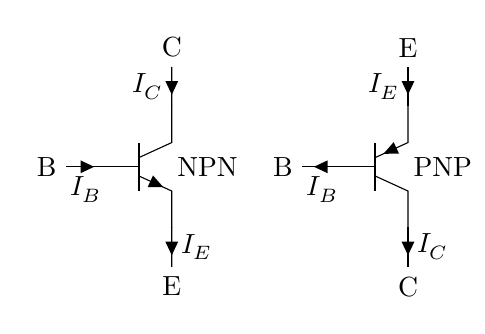
\begin{tikzpicture}
      % NPN
      \draw (0,0) node[npn, below](npn){NPN};
      \draw (npn.E) to[short, i=$I_E$] ++(0,-0.5) node[below] {E};
      \draw (npn.C) to[short, i<=$I_C$] ++(0,+0.5) node[above] {C};
      \draw (npn.B) to[short, i<=$I_B$] ++(-0.5,0) node[left] {B};
      % PNP
      \draw (3,0) node[pnp, below](pnp){PNP};
      \draw (pnp.E) to[short, i<=$I_E$] ++(0,0.5) node[above] {E};
      \draw (pnp.C) to[short, i=$I_C$] ++(0,-0.5) node[below] {C};
      \draw (pnp.B) to[short, i=$I_B$] ++(-0.5,0) node[left] {B};
    \end{tikzpicture}
  \end{center}

  \paragraph{MOSFET's}
  \begin{center}
    \ctikzset{tripoles/mos style/arrows}
    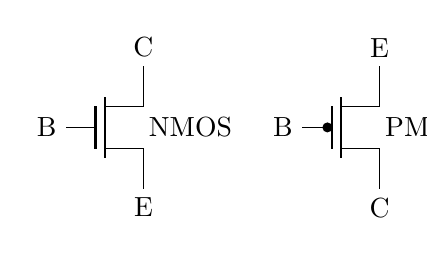
\begin{tikzpicture}
      % NMOS
      \draw (0,0) node[nmos, below](nmos){NMOS};
      \draw (nmos.E) node[below] {E};
      \draw (nmos.C) node[above] {C};
      \draw (nmos.B)  node[left] {B};
      % PMOS
      \draw (3,0) node[pmos, below](pmos){PMOS};
      \draw (pmos.E) node[above] {E};
      \draw (pmos.C) node[below] {C};
      \draw (pmos.B)  node[left] {B};
    \end{tikzpicture}
  \end{center}
  MESFET's are drawn whithout the arrow. If there is no connection
between the body and the source, the following symbols can be used:
  \begin{center}
    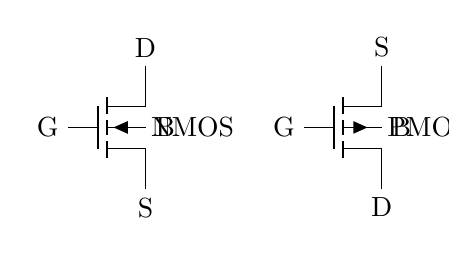
\begin{tikzpicture}
      % NMOS
      \draw (0,0) node[nfet, below](nmos){NMOS};
      \draw (nmos.S) node[below] {S};
      \draw (nmos.D) node[above] {D};
      \draw (nmos.B)  node[right] {B};
      \draw (nmos.G)  node[left] {G};
      % PMOS
      \draw (3,0) node[pfet, below](pmos){PMOS};
      \draw (pmos.S) node[above] {S};
      \draw (pmos.D) node[below] {D};
      \draw (pmos.B)  node[right] {B};
      \draw (pmos.G)  node[left] {G};
    \end{tikzpicture}
  \end{center}

  If it is an depletion device, a solid channel is drawn below the big
  line, from source to drain.

  Lastly, the JFET's:
  \begin{center}
    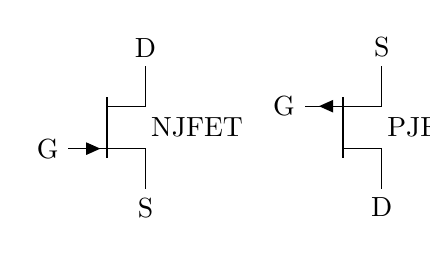
\begin{tikzpicture}
      % NMOS
      \draw (0,0) node[njfet, below](nmos){NJFET};
      \draw (nmos.S) node[below] {S};
      \draw (nmos.D) node[above] {D};
      \draw (nmos.G)  node[left] {G};
      % PMOS
      \draw (3,0) node[pjfet, below](pmos){PJFET};
      \draw (pmos.S) node[above] {S};
      \draw (pmos.D) node[below] {D};
      \draw (pmos.G)  node[left] {G};
    \end{tikzpicture}
  \end{center}



\end{multicols}


\end{document}
